\chapter{Converge cluster}

Nedenfor ses et afhængighedstræ over de forskellige enheder som systemet består af og viser samtidig enheders afhængighed med andre enheder.

\begin{figure}[ht]
    \centering
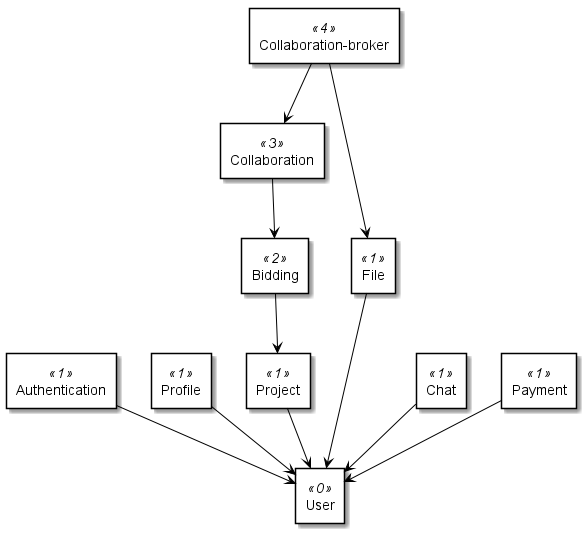
\includegraphics[width=0.6\textwidth]{diagrams/out/src/integrationstest/dependencieTree/step_0_dependencieTree/step_0_dependencieTree.png}
\caption{Viser registerings side}
\label{fig:figure2}
\end{figure}


Figur(2.1) viser afhængighedstræ over de forskellige services, som Converge cluster indeholder. Der skal dog siges at alle services benytter Authentication, samt alle services har deres egen database.
Derudover var der i gruppen reflekteret en del over hvilken test type eller tilgang der skulle benyttes til at udfør integrationstesten. Der findes forskellige former for tilgang til at udfører integrationstest, dog faldt valget over Bottom up tilgang. I Bottom Up tilgang testes hvert modul på lavere niveauer med højere moduler og bevæger sig op ad, indtil alle moduler er testet. I denne tilgang kan fejl lokaliseres nemt og at udvikling og test udføres sammen, så produktet eller applikationen er effektiv og i henhold til for eksempel kundens specifikationer. 
Herudover kan der ses på figur(2.1) at de forskellige niveauer har fået tildelt et nummer og nummeret indikerer hvor langt ned ligger de forskellige moduler (0 er det laveste modul). 

\newpage


\begin{figure}[ht]
    \centering
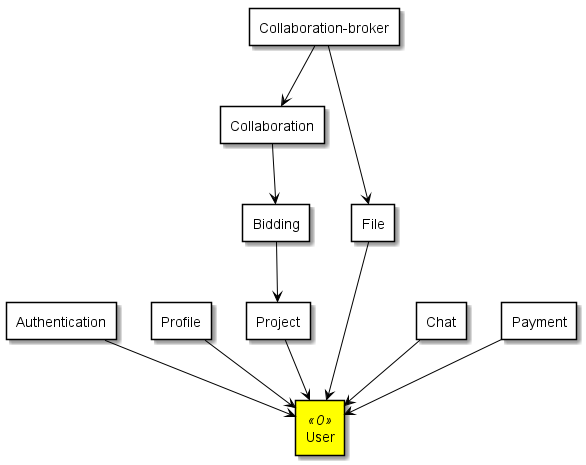
\includegraphics[width=0.6\textwidth]{diagrams/out/src/integrationstest/dependencieTree/step_1_dependencieTree/step_1_dependencieTree.png}
\caption{Viser registerings side}
\label{fig:figure2}
\end{figure}

Figur(2.2) viser det første skridt i integration testen, hvor det er user service der testes. Her bliver kaldt de forskellige metoder som der er i user service controller, herefter kaldes metoder i UserRepository, hvor der oprettes en database til netop user-servicen. 


\begin{figure}[ht]
    \centering
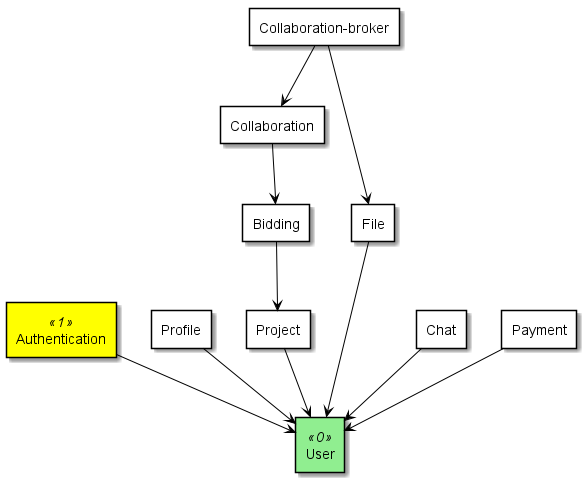
\includegraphics[width=0.6\textwidth]{diagrams/out/src/integrationstest/dependencieTree/step_2_dependencieTree/step_2_dependencieTree.png}
\caption{Viser registerings side}
\label{fig:figure2}
\end{figure}

Anden skridt er hvor der testes mellem Authentication og User, hvor testen starter ved Authentichation som kan ses på figur (2.3). Her gør man det samme som forrige skridt, hvor metoder i Authentichation service controller bliver kaldt.  

\newpage
\begin{figure}[ht]
    \centering
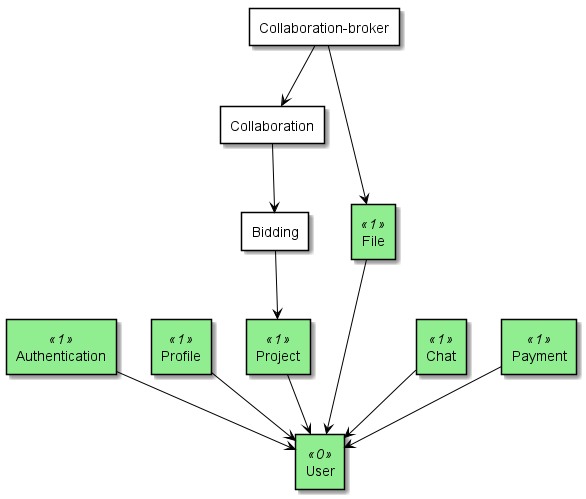
\includegraphics[width=0.6\textwidth]{diagrams/out/src/integrationstest/dependencieTree/step_3_dependencieTree/step_3_dependencieTree.png}
\caption{Viser registerings side}
\label{fig:figure2}
\end{figure}

Her sker der det samme som anden skridt, hvor alle services der ligger på niveau 1 testes ned mod User. Men her skal der bemærkes ud fra ovenstående figur at man tester med de rigtige moduler og formålet er at sikre metoder i de forskellige services fungerer som det skal og kalder de rigtige metoder til deres database.  


\begin{figure}[ht]
    \centering
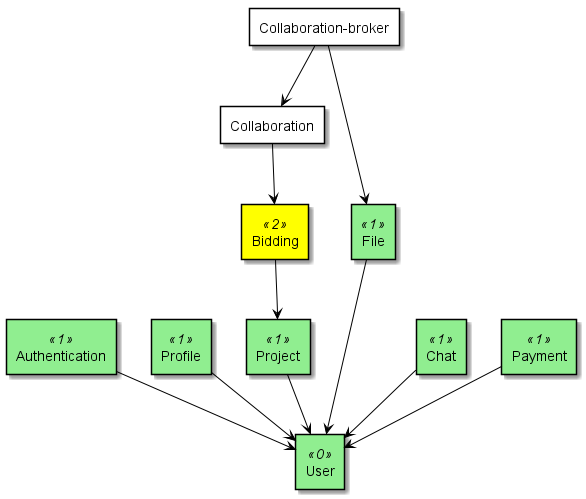
\includegraphics[width=0.6\textwidth]{diagrams/out/src/integrationstest/dependencieTree/step_4_dependencieTree/step_4_dependencieTree.png}
\caption{Viser registerings side}
\label{fig:figure2}
\end{figure}

Fjerde skridt er Bidding, hvor det er afhængige af at der er oprettet en user og et projekt for at kunne byde på det, som ses på figur(2.5). Derudover sker integrationstesten på samme måde som de forrige skridt. 

\newpage
\begin{figure}[ht]
    \centering
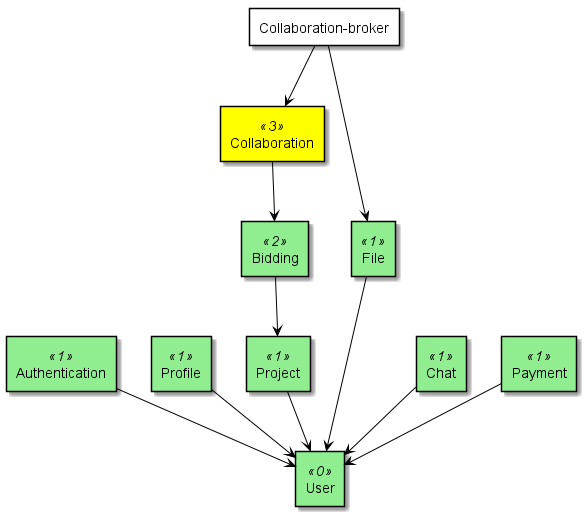
\includegraphics[width=0.6\textwidth]{diagrams/out/src/integrationstest/dependencieTree/step_5_dependencieTree/step_5_dependencieTree.png}
\caption{Viser registerings side}
\label{fig:figure2}
\end{figure}

femte skridt er Collaboration, Hvor rutens afhængighed går hele vejen ned til Project igen, som ses på figur(2.6). Derudover sker integrationstesten på samme måde som de forrige skridt. 

\begin{figure}[ht]
    \centering
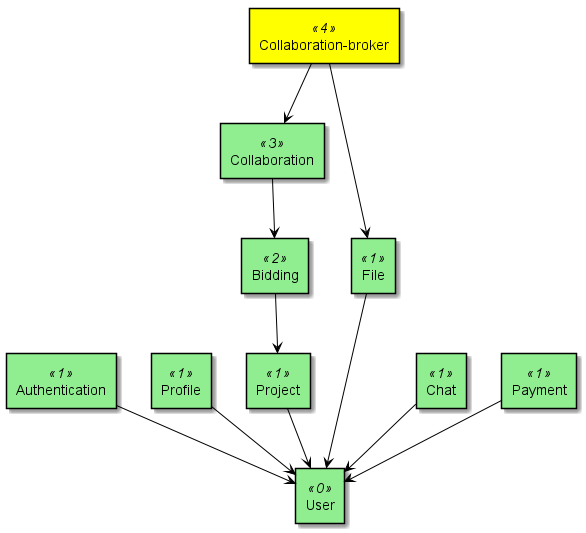
\includegraphics[width=0.6\textwidth]{diagrams/out/src/integrationstest/dependencieTree/step_6_dependencieTree/step_6_dependencieTree.png}
\caption{Viser registerings side}
\label{fig:figure2}
\end{figure}


Figur beskrivelse
Sjette skridt sker på samme måde som fjerde skrid, udover at ruten er længer og at det også er afhængig af File, som ses på figur(2.7). 


